
\documentclass[11pt,a4paper]{report}                                   

\usepackage[T1]{fontenc}
\usepackage{kpfonts}
\usepackage[utf8]{inputenc}
\usepackage[hyphens]{url}
\usepackage{graphicx}
\usepackage{a4}
\usepackage[english]{babel}
\usepackage{subfiles}
\usepackage{acronym}
\usepackage{tocbibind}
\usepackage{cmap}
\usepackage{listingsutf8}
\usepackage{color}

\newcommand{\thema}{Architektur für ein webbasiertes graphisches Modellierungsframework}
\newcommand{\schlagworte}{Modelgetriebene Softwareentwicklung, Webapplikation, Architektur}
\newcommand{\zusammenfassung}{TBD}
\newcommand{\ausgabedatum}{01.10.2017}
\newcommand{\abgabedatum}{01.04.2018}
\newcommand{\autor}{Philipp Daniels}
\newcommand{\autorStrasse}{Rheingutstraße 30}
\newcommand{\autorPLZ}{78462}
\newcommand{\autorOrt}{Konstanz}
\newcommand{\autorGeburtsort}{Mannheim}
\newcommand{\autorGeburtsdatum}{03.02.1989}
\newcommand{\prueferA}{Prof. Dr. Marko Boger}
\newcommand{\prueferB}{Prof. Dr. Markus Eiglsperger}
\newcommand{\firma}{HTWG}
\newcommand{\studiengang}{Master of Science Informatik}

%PDF linking package
\usepackage[hidelinks,breaklinks=true]{hyperref}
% hyperref customization
\hypersetup{
    pdftitle    ={\thema}, % title
    pdfsubject	={\thema}, % subject of the document
    pdfauthor	={\autor}, % author
    pdfkeywords	={}, % list of keywords
    pdfcreator	={}, % creator of the document
    pdfproducer	={}, % producer of the document
    colorlinks=false, % false: boxed links; true: colored links
    linkcolor=red, % color of internal links (change box color with linkbordercolor)
    citecolor=green, % color of links to bibliography
    filecolor=magenta, % color of file links
    urlcolor=cyan, % color of external links
    unicode=true, % non-Latin characters in Acrobat’s bookmarks
    pdftoolbar=true, % show Acrobat’s toolbar?
    pdfmenubar=true, % show Acrobat’s menu?
    pdffitwindow=false, % window fit to page when opened
    pdfnewwindow=true % links in new PDF window
}

\definecolor{lightgray}{rgb}{.9,.9,.9}
\definecolor{darkgray}{rgb}{.4,.4,.4}
\definecolor{purple}{rgb}{0.65, 0.12, 0.82}
\lstdefinelanguage{JavaScript}{
  keywords={break, case, catch, class, continue, const, constructor, debugger, default, delete, do, else, export, false, finally, for, function, get, if, import, in, instanceof, let, new, null, return, switch, this, throw, true, try, typeof, var, void, while},
  morecomment=[l]{//},
  morecomment=[s]{/*}{*/},
  morestring=[b]',
  morestring=[b]",
  keywordstyle=\color{blue}\bfseries,
  identifierstyle=\color{black},
  commentstyle=\color{purple}\ttfamily,
  stringstyle=\color{red}\ttfamily,
  sensitive=true
}

\lstset{
    basicstyle=\footnotesize,
    breakatwhitespace=false,
    breaklines=true,
    captionpos=b,
    frame=single,
    keepspaces=true,
    numbers=left,
    numbersep=5pt,
    showspaces=false,
    showstringspaces=false,
    showtabs=false,
    stepnumber=1,
    tabsize=2,
    title=\lstname,
    inputencoding=utf8/latin1
}

\newcommand{\theHchoice}{\arabic{question}.\arabic{choice}}

\begin{document}

\hypersetup{pageanchor=false}


\begin{titlepage}

\vspace*{-3.5cm}

\begin{flushleft}
\hspace*{-1cm} 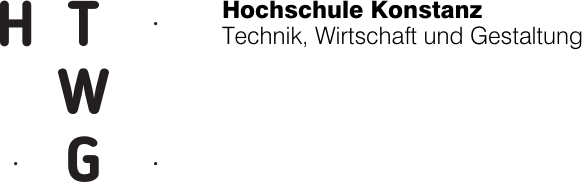
\includegraphics[width=10cm]{htwg-logo.png}
\end{flushleft}

\vspace{2.5cm}

\begin{center}
	\huge{
		\textbf{\thema} \\[5cm]
	}
	\Large{
		\textbf{\autor}} \\[6.5cm]
	\large{
		\textbf{Konstanz, \abgabedatum} \\[2.3cm]
	}
	
	\Huge{
		\textbf{{\sf MASTERARBEIT}}
	}
\end{center}

\end{titlepage}

\thispagestyle{empty}
{
\setlength{\parskip}{0.5cm}
        \begin{center}
        \textbf{\huge MASTERARBEIT}

        \textbf{zur Erlangung des akademischen Grades}

        \textbf{\Large Master of Science (M. Sc.)}

        \textbf{an der}

        \textsf{\huge Hochschule Konstanz}\\
        {\small Technik, Wirtschaft und Gestaltung}

        \textsf{\Large Fakultät Informatik} \\
        Studiengang \studiengang
        \end{center}
}
\begin{center}

\vspace*{2cm}

\begin{tabular}{p{3cm}p{10cm}}
Thema: & \textbf{\large \thema} \\[15ex]
Masterkandidat: & \autor, \autorStrasse, \autorPLZ\ \autorOrt \\[15ex]
1. Prüfer: & \prueferA \\
2. Prüfer: & \prueferB \\[25ex]
Ausgabedatum: & \ausgabedatum \\
Abgabedatum: & \abgabedatum \\
\end{tabular}
\end{center}


\hypersetup{pageanchor=true}
\pagenumbering{Roman} 
\setcounter{page}{1}


\chapter*{
  \begin{center}
  {\Large{Zusammenfassung (Abstract)}}
  \addcontentsline{toc}{chapter}{Abstract}
  \end{center}
}

\bigskip

\begin{center}
	\begin{tabular}{p{2.8cm}p{10cm}}
		Thema: & \thema \\
		 & \\
		Masterkandidat: & \autor \\
		 & \\
		Firma: & \firma \\
		 & \\
		Betreuer: & \prueferA  \\[.5ex]
		 &  \prueferB \\
		 & \\
		Abgabedatum: & \abgabedatum \\
		 & \\
		Schlagworte: & \schlagworte \\
		 & \\
	\end{tabular}
\end{center}

\bigskip

\noindent
\zusammenfassung

%
% TABLE OF CONTENTS
%
\renewcommand{\contentsname}{Inhaltsverzeichnis}
\tableofcontents
\thispagestyle{plain}
\newpage

\chapter*{Abkürzungsverzeichnis}
\label{chap:ACRONYM}
\addcontentsline{toc}{chapter}{Abkürzungsverzeichnis}

\begin{acronym}[Bash]
  \acro{lxc}[LXC]{Linux Container}
  \acro{vm}[VM]{Virtual Machine}

\end{acronym}

\newpage

\label{chap:FIGURES}
\renewcommand\listfigurename{Abbildungsverzeichnis}
\listoffigures
\newpage


\label{chap:LIST_OF_LISTINGS}
\renewcommand\lstlistlistingname{Quelltextverzeichnis}
\lstlistoflistings
\newpage



%Content
\pagenumbering{arabic} 
\setcounter{page}{1}
\setlength{\parindent}{0em}
\setlength{\parskip}{1em}
\renewcommand{\baselinestretch}{1.5}
\renewcommand\chaptername{Kapitel}
\chapter{Einleitung}
\label{sec:INTRO}

\section{Problemstellung}
\label{sec:INTRO_PROBLEM}

\section{Wissenschaftliche Fragestellung}
\label{sec:INTRO_SCIENTIFIC_QUESTION}

\section{Aufbau}
\label{sec:INTRO_STRUCTURE}


\chapter{Ausgangssituation}
\label{sec:STATE_OF_THE_ART}


\chapter{Lösung}
\label{sec:SOLUTION}

\section{Modellierungsframework}
\label{sec:SOLUTION_MODEL}

\section{Webapplikation}
\label{sec:SOLUTION_WEB}

\section{Zeta}
\label{sec:SOLUTION_ZETA}


\chapter{Resümee}
\label{sec:SUMMARY}

\section{Schlussfolgerungen}
\label{sec:SUMMARY_CONCLUSION}

\section{Ausblick}
\label{sec:SUMMARY_OUTLOOK}



\renewcommand\thesection{A.\arabic{section}}
\renewcommand\thesubsection{\thesection.\arabic{subsection}}

\chapter*{Anhänge}
\label{chap:APPENDIX}
\addcontentsline{toc}{chapter}{Anhänge}

\pagenumbering{arabic}
\setcounter{page}{1}
\renewcommand{\thepage}{A-\arabic{page}}


\section{Abbildungen}
\label{sec:APPENDIX_FIGURES}

\section{Quelltexte}
\label{sec:APPENDIX_LISTINGS}

\renewcommand{\baselinestretch}{1}

\clearpage


\phantomsection
\renewcommand{\bibname}{Quellenverzeichnis}
\bibliography{references}
\bibliographystyle{apalike}
\newpage


\end{document}
